\documentclass[11pt]{article}

% Review version for ACL Rolling Review
\usepackage[review]{acl}

% Standard ACL packages
\usepackage{times}
\usepackage{latexsym}

% Encoding
\usepackage[T1]{fontenc}
\usepackage[utf8]{inputenc}
% Typography
\usepackage{microtype}
\usepackage{inconsolata}
\usepackage{amsmath,amssymb,mathtools}
\usepackage{booktabs}
\usepackage{multirow}
\usepackage{array}
\usepackage{tabularx}
\usepackage{graphicx}
\usepackage{adjustbox}
\usepackage{tikz}
\usetikzlibrary{backgrounds,calc}
\usepackage[nameinlink,noabbrev]{cleveref}

% xcolor is already loaded by acl.sty
\definecolor{categoryyellow}{RGB}{255,255,204}
\definecolor{categoryblue}{RGB}{207,226,251}
\definecolor{categorygreen}{RGB}{226,240,220}
\definecolor{referencegray}{RGB}{248,248,248}
\definecolor{referenceblue}{RGB}{0,0,128}

\newcommand{\mstd}[2]{#1$_{\pm #2}$}
\newcommand{\best}[1]{\textbf{#1}}


% A real BibTeX citation is issued for every paper shown in the taxonomy.
\newcommand{\taxpaper}[2]{#1~{\color{referenceblue}\citep{#2}}}

% name, x, y, width, height, text
\newcommand{\refbox}[6]{%
  \node[references,
        text width=\dimexpr#4pt-5pt\relax,
        minimum width=#4pt,
        minimum height=#5pt]
        (#1) at (#2,#3) {#6};%
}

% name, x, y, width, height, fill, text
\newcommand{\labelbox}[7]{%
  \node[labelbox,fill=#6,
        text width=\dimexpr#4pt-5pt\relax,
        minimum width=#4pt,
        minimum height=#5pt]
        (#1) at (#2,#3) {#7};%
}


\title{Human--AI Alignment: A Survey of Specification, Supervision, Mechanisms, and Assurance}

\author{
  First Author \\
  Affiliation \\
  \texttt{email@example.com}
}

\begin{document}

\title{A Survey on Human--AI Alignment: Taxonomy, Methods, and Challenges}

\author{
  First Author \\
  Affiliation \\
  \texttt{email@example.com}
}

\maketitle

\begin{abstract}
Human--AI alignment spans training, inference, adaptation, and deployment, yet research on targets, feedback, interventions, and evaluation remains fragmented. We organize the field as an iterative lifecycle of \emph{specification}, \emph{supervision}, \emph{mechanisms}, and \emph{assurance}. The survey examines how targets and stakeholders are defined, how human, AI, and verifiable feedback is represented, how training- and inference-time methods shape behavior, and how alignment is evaluated and preserved after deployment. This lifecycle view connects challenges in heterogeneous and evolving preferences, scalable oversight, evaluator reliability, and post-adaptation alignment. An actively maintained repository accompanies the survey at \url{https://github.com/Thang1703hrsh/Awesome-Human-AI-Alignment}.
\end{abstract}

\section{Introduction}
\label{sec:introduction}

The rapid development of foundation models has broadened Human--AI alignment from post-training preference optimization to a problem spanning training, inference, adaptation, and deployment. Aligned systems must follow instructions and preferences, satisfy safety constraints, accommodate heterogeneous users, remain controllable during interaction, and preserve desired behavior after modification \citep{christiano2017preferences,ouyang2022instructgpt,bai2022constitutional,rafailov2023dpo,qi2024finetuning}. Yet these requirements are often studied separately as objectives, feedback sources, optimization methods, or evaluation problems, obscuring their dependencies and how failures propagate across stages.

\begin{figure}[t]
    \centering
    \includegraphics[width=\columnwidth]{Human_AI_Alignment.pdf}
    \caption{The Human--AI Alignment lifecycle. Alignment proceeds through specification, supervision, mechanisms, and assurance, with deployment feedback enabling iterative revision.}
    \label{fig:human-ai-alignment-lifecycle}
\end{figure}

We organize this literature as an iterative functional lifecycle, illustrated in Figure~\ref{fig:human-ai-alignment-lifecycle}, around four questions. \emph{What should be aligned, and whose requirements define the target?} Alignment Specification identifies desired behavior, constraints, and stakeholders. \emph{How is the target observed?} Alignment Supervision covers the sources, representations, and reliability of feedback. \emph{How is behavior shaped?} Alignment Mechanisms translate this evidence into training- or inference-time interventions. \emph{How do we know alignment holds?} Alignment Assurance evaluates behavior, robustness, preservation, and deployment-time evidence. Assurance findings can revise earlier stages, making the lifecycle iterative rather than a one-shot pipeline.

Figure~\ref{fig:human-ai-alignment-taxonomy} summarizes the resulting taxonomy. Its categories denote functional contributions rather than mutually exclusive paper classes, allowing a study to contribute to multiple lifecycle stages. This perspective captures settings in which preferences vary across stakeholders \citep{sorensen2024pluralistic,siththaranjan2024distributional}, supervision combines learned and verifiable signals \citep{mu2024rulebased,lightman2024verify}, or interventions span training and inference \citep{rimsky2024caa,greenblatt2024control}.

\begin{figure*}[p]
\centering
\begingroup
\providecommand{\taxpaper}[2]{#1~{\color{referenceblue}\citep{#2}}}
\begin{adjustbox}{max width=\textwidth,max totalheight=.86\textheight,center,keepaspectratio}
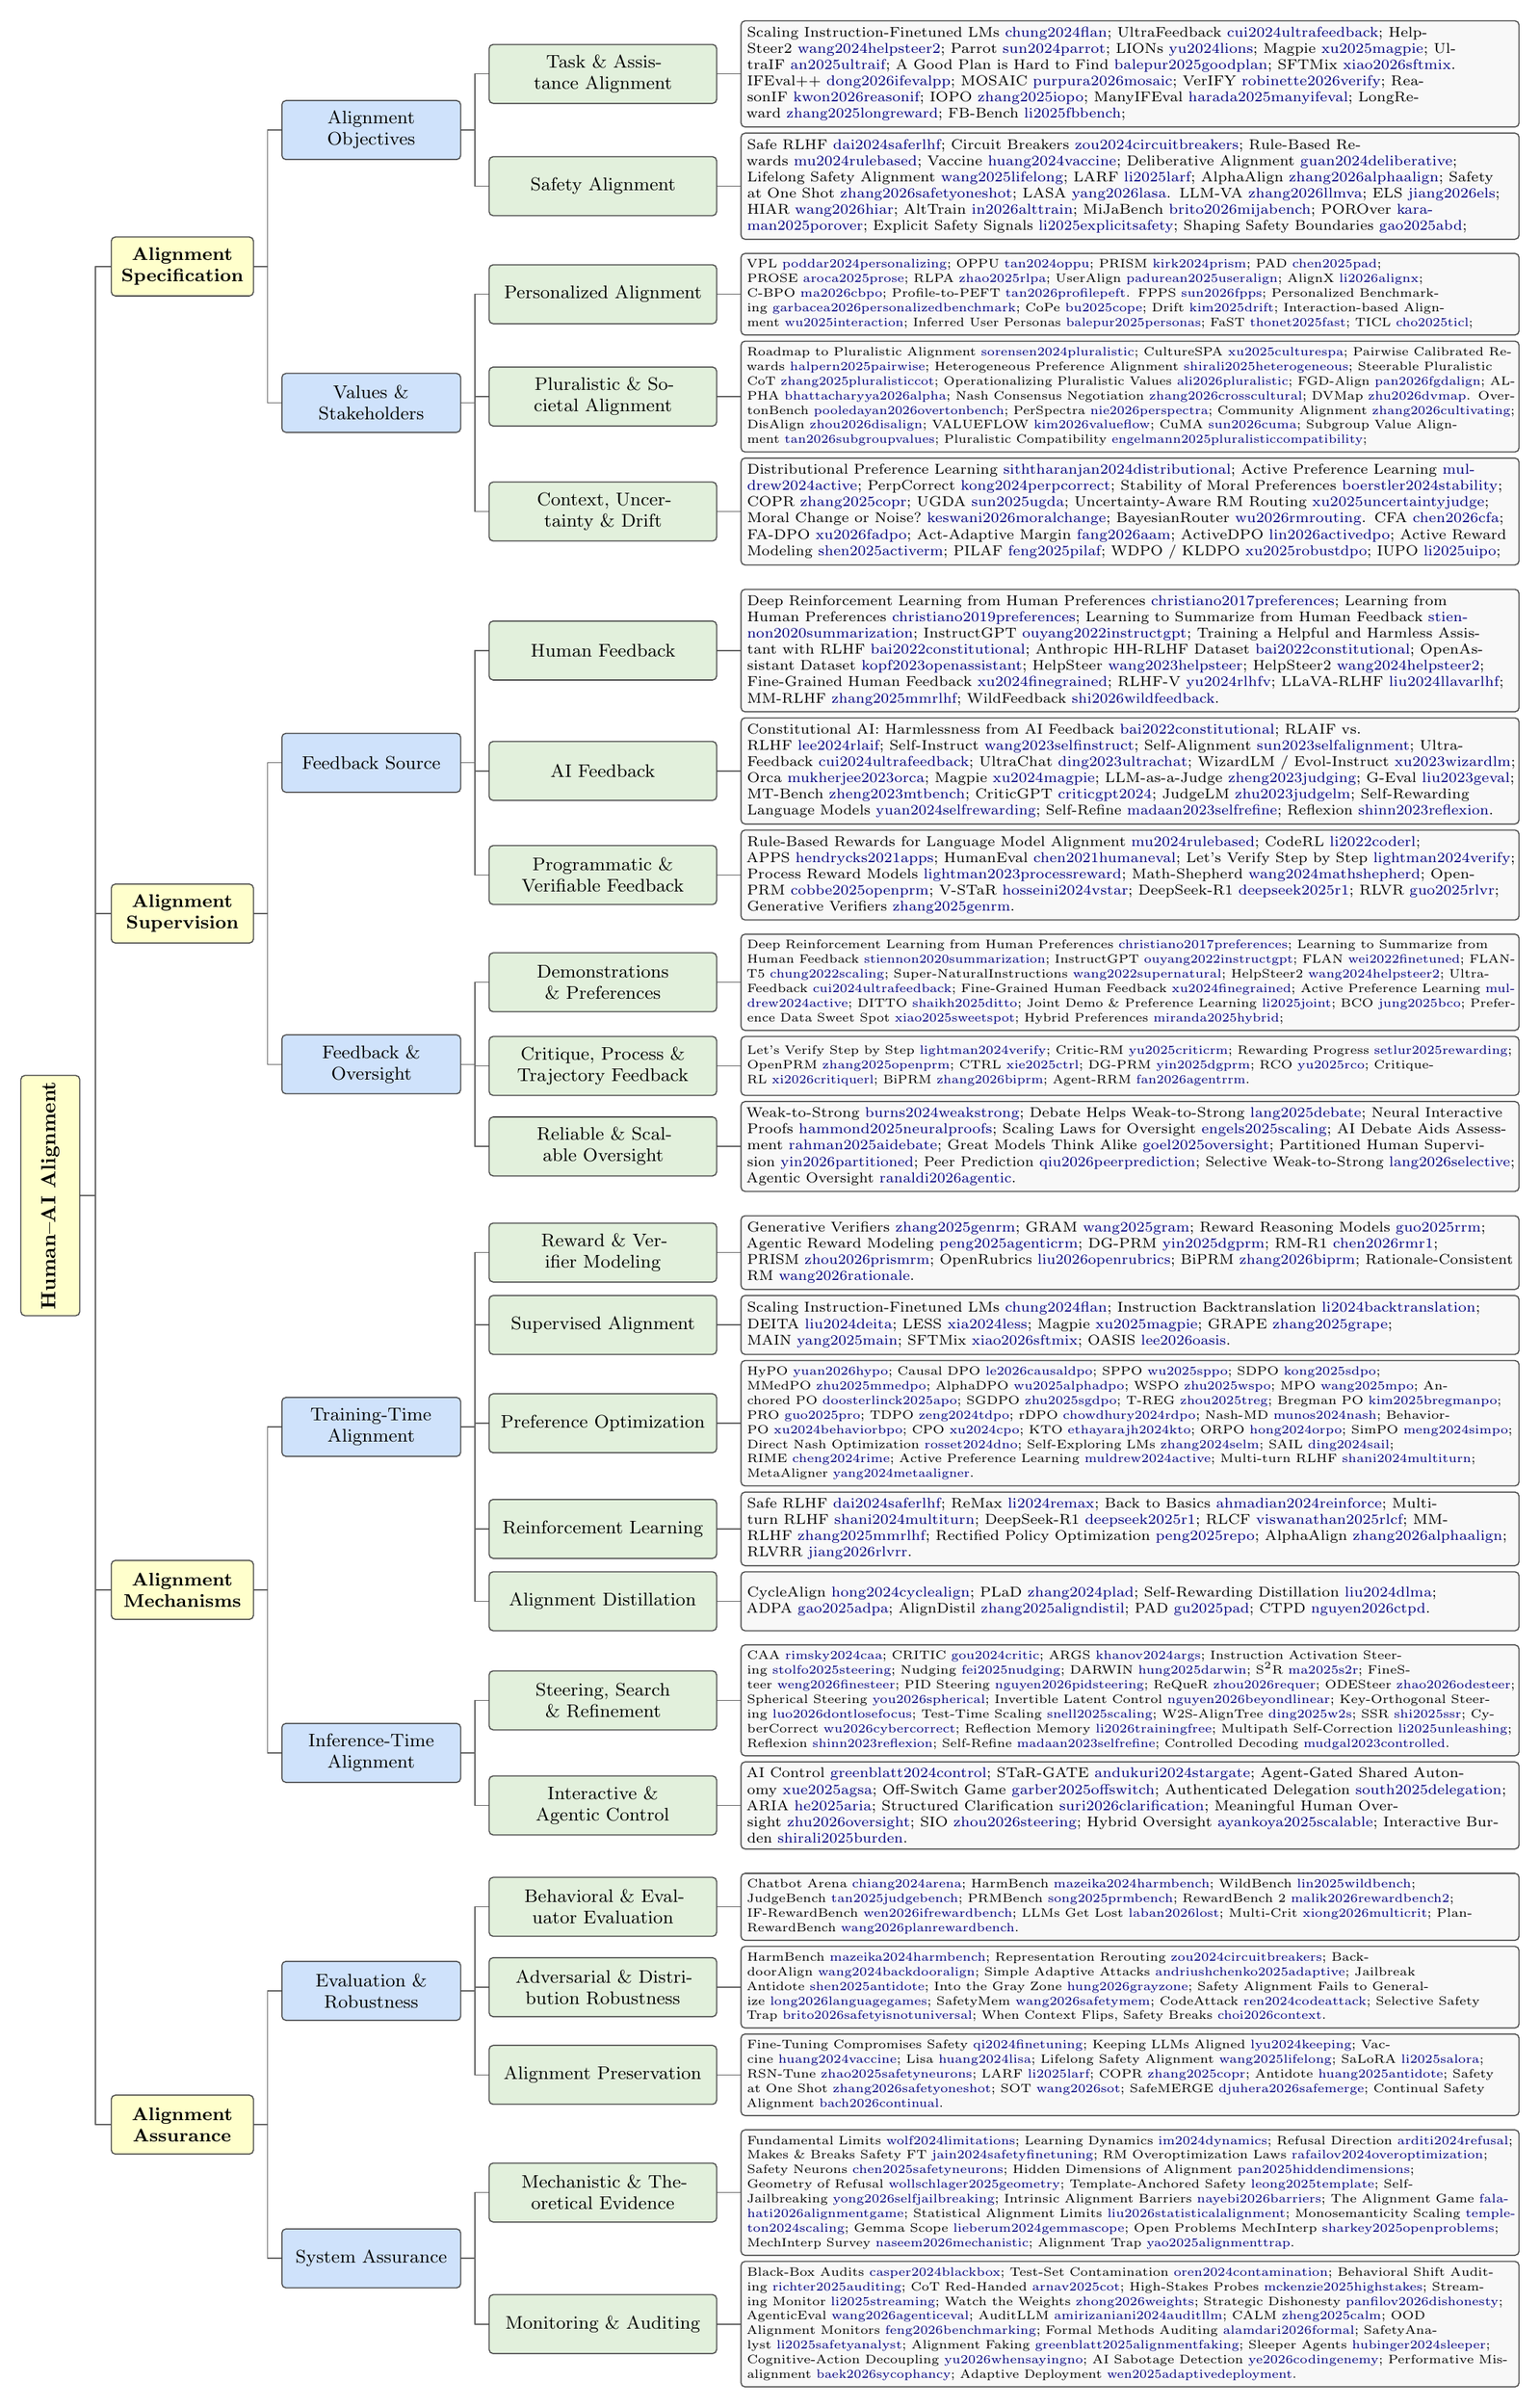
\begin{tikzpicture}[x=1pt,y=-1pt,box/.style={draw=black!70,line width=.55pt,rounded corners=2pt,inner xsep=3pt,inner ysep=3pt,outer sep=0pt,align=center,font=\fontsize{9}{10.5}\selectfont},refs/.style={box,fill=referencegray,align=left,text width=377pt,minimum width=383pt,minimum height=29pt,font=\fontsize{8}{9.5}\selectfont},refsDense/.style={refs,font=\fontsize{6.8}{8.0}\selectfont},refsUltraDense/.style={refs,font=\fontsize{6.2}{7.2}\selectfont},branch/.style={draw=black!60,line width=.55pt,line cap=round,line join=round}]
\def\RowGap{3pt}\def\GroupGap{7pt}\def\PillarGap{12pt}
% =========================================================
% I. ALIGNMENT SPECIFICATION
% =========================================================

\node[refsDense,anchor=north] (refTaskAssistance) at (536.5,0) {\taxpaper{Scaling Instruction-Finetuned LMs}{chung2024flan}; \taxpaper{UltraFeedback}{cui2024ultrafeedback}; \taxpaper{HelpSteer2}{wang2024helpsteer2}; \taxpaper{Parrot}{sun2024parrot}; \taxpaper{LIONs}{yu2024lions}; \taxpaper{Magpie}{xu2025magpie}; \taxpaper{UltraIF}{an2025ultraif}; \taxpaper{A Good Plan is Hard to Find}{balepur2025goodplan}; \taxpaper{SFTMix}{xiao2026sftmix}. \taxpaper{IFEval++}{dong2026ifevalpp}; \taxpaper{MOSAIC}{purpura2026mosaic}; \taxpaper{VerIFY}{robinette2026verify}; \taxpaper{ReasonIF}{kwon2026reasonif}; \taxpaper{IOPO}{zhang2025iopo}; \taxpaper{ManyIFEval}{harada2025manyifeval}; \taxpaper{LongReward}{zhang2025longreward}; \taxpaper{FB-Bench}{li2025fbbench};};
\node[box,fill=categorygreen,text width=106pt,minimum width=112pt,minimum height=29pt] (taskAssistance) at (277,0 |- refTaskAssistance.center) {Task \& Assistance Alignment};

\node[refsDense,anchor=north] (refSafetyAlignment) at ([yshift=-\RowGap]refTaskAssistance.south) {\taxpaper{Safe RLHF}{dai2024saferlhf}; \taxpaper{Circuit Breakers}{zou2024circuitbreakers}; \taxpaper{Rule-Based Rewards}{mu2024rulebased}; \taxpaper{Vaccine}{huang2024vaccine}; \taxpaper{Deliberative Alignment}{guan2024deliberative}; \taxpaper{Lifelong Safety Alignment}{wang2025lifelong}; \taxpaper{LARF}{li2025larf}; \taxpaper{AlphaAlign}{zhang2026alphaalign}; \taxpaper{Safety at One Shot}{zhang2026safetyoneshot}; \taxpaper{LASA}{yang2026lasa}. \taxpaper{LLM-VA}{zhang2026llmva}; \taxpaper{ELS}{jiang2026els}; \taxpaper{HIAR}{wang2026hiar}; \taxpaper{AltTrain}{in2026alttrain}; \taxpaper{MiJaBench}{brito2026mijabench}; \taxpaper{POROver}{karaman2025porover}; \taxpaper{Explicit Safety Signals}{li2025explicitsafety}; \taxpaper{Shaping Safety Boundaries}{gao2025abd};};
\node[box,fill=categorygreen,text width=106pt,minimum width=112pt,minimum height=29pt] (safetyAlignment) at (277,0 |- refSafetyAlignment.center) {Safety Alignment};
\coordinate (alignmentObjectivesMid) at ($(taskAssistance.center)!0.5!(safetyAlignment.center)$);
\node[box,fill=categoryblue,text width=82pt,minimum width=88pt,minimum height=29pt] (alignmentObjectives) at (163,0 |- alignmentObjectivesMid) {Alignment Objectives};

\node[refsUltraDense,anchor=north] (refPersonalized) at ([yshift=-\GroupGap]refSafetyAlignment.south) {\taxpaper{VPL}{poddar2024personalizing}; \taxpaper{OPPU}{tan2024oppu}; \taxpaper{PRISM}{kirk2024prism}; \taxpaper{PAD}{chen2025pad}; \taxpaper{PROSE}{aroca2025prose}; \taxpaper{RLPA}{zhao2025rlpa}; \taxpaper{UserAlign}{padurean2025useralign}; \taxpaper{AlignX}{li2026alignx}; \taxpaper{C-BPO}{ma2026cbpo}; \taxpaper{Profile-to-PEFT}{tan2026profilepeft}. \taxpaper{FPPS}{sun2026fpps}; \taxpaper{Personalized Benchmarking}{garbacea2026personalizedbenchmark}; \taxpaper{CoPe}{bu2025cope}; \taxpaper{Drift}{kim2025drift}; \taxpaper{Interaction-based Alignment}{wu2025interaction}; \taxpaper{Inferred User Personas}{balepur2025personas}; \taxpaper{FaST}{thonet2025fast}; \taxpaper{TICL}{cho2025ticl};};
\node[box,fill=categorygreen,text width=106pt,minimum width=112pt,minimum height=29pt] (personalized) at (277,0 |- refPersonalized.center) {Personalized Alignment};

\node[refsUltraDense,anchor=north] (refPluralistic) at ([yshift=-\RowGap]refPersonalized.south) {\taxpaper{Roadmap to Pluralistic Alignment}{sorensen2024pluralistic}; \taxpaper{CultureSPA}{xu2025culturespa}; \taxpaper{Pairwise Calibrated Rewards}{halpern2025pairwise}; \taxpaper{Heterogeneous Preference Alignment}{shirali2025heterogeneous}; \taxpaper{Steerable Pluralistic CoT}{zhang2025pluralisticcot}; \taxpaper{Operationalizing Pluralistic Values}{ali2026pluralistic}; \taxpaper{FGD-Align}{pan2026fgdalign}; \taxpaper{ALPHA}{bhattacharyya2026alpha}; \taxpaper{Nash Consensus Negotiation}{zhang2026crosscultural}; \taxpaper{DVMap}{zhu2026dvmap}. \taxpaper{OvertonBench}{pooledayan2026overtonbench}; \taxpaper{PerSpectra}{nie2026perspectra}; \taxpaper{Community Alignment}{zhang2026cultivating}; \taxpaper{DisAlign}{zhou2026disalign}; \taxpaper{VALUEFLOW}{kim2026valueflow}; \taxpaper{CuMA}{sun2026cuma}; \taxpaper{Subgroup Value Alignment}{tan2026subgroupvalues}; \taxpaper{Pluralistic Compatibility}{engelmann2025pluralisticcompatibility};};
\node[box,fill=categorygreen,text width=106pt,minimum width=112pt,minimum height=29pt] (pluralistic) at (277,0 |- refPluralistic.center) {Pluralistic \& Societal Alignment};

\node[refsDense,anchor=north] (refContextUncertaintyDrift) at ([yshift=-\RowGap]refPluralistic.south) {\taxpaper{Distributional Preference Learning}{siththaranjan2024distributional}; \taxpaper{Active Preference Learning}{muldrew2024active}; \taxpaper{PerpCorrect}{kong2024perpcorrect}; \taxpaper{Stability of Moral Preferences}{boerstler2024stability}; \taxpaper{COPR}{zhang2025copr}; \taxpaper{UGDA}{sun2025ugda}; \taxpaper{Uncertainty-Aware RM Routing}{xu2025uncertaintyjudge}; \taxpaper{Moral Change or Noise?}{keswani2026moralchange}; \taxpaper{BayesianRouter}{wu2026rmrouting}. \taxpaper{CFA}{chen2026cfa}; \taxpaper{FA-DPO}{xu2026fadpo}; \taxpaper{Act-Adaptive Margin}{fang2026aam}; \taxpaper{ActiveDPO}{lin2026activedpo}; \taxpaper{Active Reward Modeling}{shen2025activerm}; \taxpaper{PILAF}{feng2025pilaf}; \taxpaper{WDPO / KLDPO}{xu2025robustdpo}; \taxpaper{IUPO}{li2025uipo};};
\node[box,fill=categorygreen,text width=106pt,minimum width=112pt,minimum height=29pt] (contextUncertaintyDrift) at (277,0 |- refContextUncertaintyDrift.center) {Context, Uncertainty \& Drift};
\coordinate (valuesStakeholdersMid) at ($(personalized.center)!0.5!(contextUncertaintyDrift.center)$);
\node[box,fill=categoryblue,text width=82pt,minimum width=88pt,minimum height=29pt] (valuesStakeholders) at (163,0 |- valuesStakeholdersMid) {Values \& Stakeholders};
\coordinate (specificationMid) at ($(alignmentObjectives.center)!0.5!(valuesStakeholders.center)$);
\node[box,fill=categoryyellow,text width=64pt,minimum width=70pt,minimum height=29pt] (pillarSpecification) at (70,0 |- specificationMid) {\textbf{Alignment\\Specification}};

% =========================================================
% II. ALIGNMENT SUPERVISION
% =========================================================

\node[refsDense,anchor=north] (refHumanFeedback) at ([yshift=-\PillarGap]refContextUncertaintyDrift.south) 
{
\taxpaper{Deep Reinforcement Learning from Human Preferences}{christiano2017preferences};
\taxpaper{Learning from Human Preferences}{christiano2019preferences};
\taxpaper{Learning to Summarize from Human Feedback}{stiennon2020summarization};
\taxpaper{InstructGPT}{ouyang2022instructgpt};
\taxpaper{Training a Helpful and Harmless Assistant with RLHF}{bai2022constitutional};
\taxpaper{Anthropic HH-RLHF Dataset}{bai2022constitutional};
\taxpaper{OpenAssistant Dataset}{kopf2023openassistant};
\taxpaper{HelpSteer}{wang2023helpsteer};
\taxpaper{HelpSteer2}{wang2024helpsteer2};
\taxpaper{Fine-Grained Human Feedback}{xu2024finegrained};
\taxpaper{RLHF-V}{yu2024rlhfv};
\taxpaper{LLaVA-RLHF}{liu2024llavarlhf};
\taxpaper{MM-RLHF}{zhang2025mmrlhf};
\taxpaper{WildFeedback}{shi2026wildfeedback}.
};

\node[box,fill=categorygreen,text width=106pt,minimum width=112pt,minimum height=29pt] 
(humanFeedback) at (277,0 |- refHumanFeedback.center) 
{Human Feedback};


\node[refsDense,anchor=north] (refAIFeedback) at ([yshift=-\RowGap]refHumanFeedback.south) 
{
\taxpaper{Constitutional AI: Harmlessness from AI Feedback}{bai2022constitutional};
\taxpaper{RLAIF vs. RLHF}{lee2024rlaif};
\taxpaper{Self-Instruct}{wang2023selfinstruct};
\taxpaper{Self-Alignment}{sun2023selfalignment};
\taxpaper{UltraFeedback}{cui2024ultrafeedback};
\taxpaper{UltraChat}{ding2023ultrachat};
\taxpaper{WizardLM / Evol-Instruct}{xu2023wizardlm};
\taxpaper{Orca}{mukherjee2023orca};
\taxpaper{Magpie}{xu2024magpie};
\taxpaper{LLM-as-a-Judge}{zheng2023judging};
\taxpaper{G-Eval}{liu2023geval};
\taxpaper{MT-Bench}{zheng2023mtbench};
\taxpaper{CriticGPT}{criticgpt2024};
\taxpaper{JudgeLM}{zhu2023judgelm};
\taxpaper{Self-Rewarding Language Models}{yuan2024selfrewarding};
\taxpaper{Self-Refine}{madaan2023selfrefine};
\taxpaper{Reflexion}{shinn2023reflexion}.
};

\node[box,fill=categorygreen,text width=106pt,minimum width=112pt,minimum height=29pt] 
(aiFeedback) at (277,0 |- refAIFeedback.center) 
{AI Feedback};


\node[refsDense,anchor=north] (refProgrammaticVerifiable) at ([yshift=-\RowGap]refAIFeedback.south) 
{
\taxpaper{Rule-Based Rewards for Language Model Alignment}{mu2024rulebased};
\taxpaper{CodeRL}{li2022coderl};
\taxpaper{APPS}{hendrycks2021apps};
\taxpaper{HumanEval}{chen2021humaneval};
\taxpaper{Let's Verify Step by Step}{lightman2024verify};
\taxpaper{Process Reward Models}{lightman2023processreward};
\taxpaper{Math-Shepherd}{wang2024mathshepherd};
\taxpaper{OpenPRM}{cobbe2025openprm};
\taxpaper{V-STaR}{hosseini2024vstar};
\taxpaper{DeepSeek-R1}{deepseek2025r1};
\taxpaper{RLVR}{guo2025rlvr};
\taxpaper{Generative Verifiers}{zhang2025genrm}.
};

\node[box,fill=categorygreen,text width=106pt,minimum width=112pt,minimum height=29pt] 
(programmaticVerifiable) at (277,0 |- refProgrammaticVerifiable.center) 
{Programmatic \& Verifiable Feedback};


\coordinate (feedbackSourceMid) 
at ($(humanFeedback.center)!0.5!(programmaticVerifiable.center)$);

\node[box,fill=categoryblue,text width=82pt,minimum width=88pt,minimum height=29pt] 
(feedbackSource) at (163,0 |- feedbackSourceMid) 
{Feedback Source};

\node[refsUltraDense,anchor=north] (refDemonstrationsPreferences) at ([yshift=-\GroupGap]refProgrammaticVerifiable.south) 
{
\taxpaper{Deep Reinforcement Learning from Human Preferences}{christiano2017preferences};
\taxpaper{Learning to Summarize from Human Feedback}{stiennon2020summarization};
\taxpaper{InstructGPT}{ouyang2022instructgpt};
\taxpaper{FLAN}{wei2022finetuned};
\taxpaper{FLAN-T5}{chung2022scaling};
\taxpaper{Super-NaturalInstructions}{wang2022supernatural};
\taxpaper{HelpSteer2}{wang2024helpsteer2};
\taxpaper{UltraFeedback}{cui2024ultrafeedback};
\taxpaper{Fine-Grained Human Feedback}{xu2024finegrained};
\taxpaper{Active Preference Learning}{muldrew2024active};
\taxpaper{DITTO}{shaikh2025ditto};
\taxpaper{Joint Demo \& Preference Learning}{li2025joint};
\taxpaper{BCO}{jung2025bco};
\taxpaper{Preference Data Sweet Spot}{xiao2025sweetspot};
\taxpaper{Hybrid Preferences}{miranda2025hybrid};
};
\node[box,fill=categorygreen,text width=106pt,minimum width=112pt,minimum height=29pt] 
(demonstrationsPreferences) at (277,0 |- refDemonstrationsPreferences.center) 
{Demonstrations \& Preferences};

\node[refsUltraDense,anchor=north] (refCritiqueProcessTrajectory) at ([yshift=-\RowGap]refDemonstrationsPreferences.south) {\taxpaper{Let's Verify Step by Step}{lightman2024verify}; \taxpaper{Critic-RM}{yu2025criticrm}; \taxpaper{Rewarding Progress}{setlur2025rewarding}; \taxpaper{OpenPRM}{zhang2025openprm}; \taxpaper{CTRL}{xie2025ctrl}; \taxpaper{DG-PRM}{yin2025dgprm}; \taxpaper{RCO}{yu2025rco}; \taxpaper{Critique-RL}{xi2026critiquerl}; \taxpaper{BiPRM}{zhang2026biprm}; \taxpaper{Agent-RRM}{fan2026agentrrm}.};
\node[box,fill=categorygreen,text width=106pt,minimum width=112pt,minimum height=29pt] (critiqueProcessTrajectory) at (277,0 |- refCritiqueProcessTrajectory.center) {Critique, Process \& Trajectory Feedback};

\node[refsDense,anchor=north] (refReliableScalable) at ([yshift=-\RowGap]refCritiqueProcessTrajectory.south) {\taxpaper{Weak-to-Strong}{burns2024weakstrong}; \taxpaper{Debate Helps Weak-to-Strong}{lang2025debate}; \taxpaper{Neural Interactive Proofs}{hammond2025neuralproofs}; \taxpaper{Scaling Laws for Oversight}{engels2025scaling}; \taxpaper{AI Debate Aids Assessment}{rahman2025aidebate}; \taxpaper{Great Models Think Alike}{goel2025oversight}; \taxpaper{Partitioned Human Supervision}{yin2026partitioned}; \taxpaper{Peer Prediction}{qiu2026peerprediction}; \taxpaper{Selective Weak-to-Strong}{lang2026selective}; \taxpaper{Agentic Oversight}{ranaldi2026agentic}.};
\node[box,fill=categorygreen,text width=106pt,minimum width=112pt,minimum height=29pt] (reliableScalable) at (277,0 |- refReliableScalable.center) {Reliable \& Scalable Oversight};
\coordinate (feedbackOversightMid) at ($(demonstrationsPreferences.center)!0.5!(reliableScalable.center)$);
\node[box,fill=categoryblue,text width=82pt,minimum width=88pt,minimum height=29pt] (feedbackOversight) at (163,0 |- feedbackOversightMid) {Feedback \& Oversight};
\coordinate (supervisionMid) at ($(feedbackSource.center)!0.5!(feedbackOversight.center)$);
\node[box,fill=categoryyellow,text width=64pt,minimum width=70pt,minimum height=29pt] (pillarSupervision) at (70,0 |- supervisionMid) {\textbf{Alignment\\Supervision}};

% =========================================================
% III. ALIGNMENT MECHANISMS
% =========================================================
\node[refsDense,anchor=north] (refRewardVerifier) at ([yshift=-\PillarGap]refReliableScalable.south) {\taxpaper{Generative Verifiers}{zhang2025genrm}; \taxpaper{GRAM}{wang2025gram}; \taxpaper{Reward Reasoning Models}{guo2025rrm}; \taxpaper{Agentic Reward Modeling}{peng2025agenticrm}; \taxpaper{DG-PRM}{yin2025dgprm}; \taxpaper{RM-R1}{chen2026rmr1}; \taxpaper{PRISM}{zhou2026prismrm}; \taxpaper{OpenRubrics}{liu2026openrubrics}; \taxpaper{BiPRM}{zhang2026biprm}; \taxpaper{Rationale-Consistent RM}{wang2026rationale}.};
\node[box,fill=categorygreen,text width=106pt,minimum width=112pt,minimum height=29pt] (rewardVerifier) at (277,0 |- refRewardVerifier.center) {Reward \& Verifier Modeling};

\node[refsDense,anchor=north] (refSupervisedAlignment) at ([yshift=-\RowGap]refRewardVerifier.south) {\taxpaper{Scaling Instruction-Finetuned LMs}{chung2024flan}; \taxpaper{Instruction Backtranslation}{li2024backtranslation}; \taxpaper{DEITA}{liu2024deita}; \taxpaper{LESS}{xia2024less}; \taxpaper{Magpie}{xu2025magpie}; \taxpaper{GRAPE}{zhang2025grape}; \taxpaper{MAIN}{yang2025main}; \taxpaper{SFTMix}{xiao2026sftmix}; \taxpaper{OASIS}{lee2026oasis}.};
\node[box,fill=categorygreen,text width=106pt,minimum width=112pt,minimum height=29pt] (supervisedAlignment) at (277,0 |- refSupervisedAlignment.center) {Supervised Alignment};

\node[refsUltraDense,anchor=north] (refPreferenceOptimization) at ([yshift=-\RowGap]refSupervisedAlignment.south) {\taxpaper{HyPO}{yuan2026hypo}; \taxpaper{Causal DPO}{le2026causaldpo}; \taxpaper{SPPO}{wu2025sppo}; \taxpaper{SDPO}{kong2025sdpo}; \taxpaper{MMedPO}{zhu2025mmedpo}; \taxpaper{AlphaDPO}{wu2025alphadpo}; \taxpaper{WSPO}{zhu2025wspo}; \taxpaper{MPO}{wang2025mpo}; \taxpaper{Anchored PO}{doosterlinck2025apo}; \taxpaper{SGDPO}{zhu2025sgdpo}; \taxpaper{T-REG}{zhou2025treg}; \taxpaper{Bregman PO}{kim2025bregmanpo}; \taxpaper{PRO}{guo2025pro}; \taxpaper{TDPO}{zeng2024tdpo}; \taxpaper{rDPO}{chowdhury2024rdpo}; \taxpaper{Nash-MD}{munos2024nash}; \taxpaper{Behavior-PO}{xu2024behaviorbpo}; \taxpaper{CPO}{xu2024cpo}; \taxpaper{KTO}{ethayarajh2024kto}; \taxpaper{ORPO}{hong2024orpo}; \taxpaper{SimPO}{meng2024simpo}; \taxpaper{Direct Nash Optimization}{rosset2024dno}; \taxpaper{Self-Exploring LMs}{zhang2024selm}; \taxpaper{SAIL}{ding2024sail}; \taxpaper{RIME}{cheng2024rime}; \taxpaper{Active Preference Learning}{muldrew2024active}; \taxpaper{Multi-turn RLHF}{shani2024multiturn}; \taxpaper{MetaAligner}{yang2024metaaligner}.};
\node[box,fill=categorygreen,text width=106pt,minimum width=112pt,minimum height=29pt] (preferenceOptimization) at (277,0 |- refPreferenceOptimization.center) {Preference Optimization};

\node[refsDense,anchor=north] (refReinforcementLearning) at ([yshift=-\RowGap]refPreferenceOptimization.south) {\taxpaper{Safe RLHF}{dai2024saferlhf}; \taxpaper{ReMax}{li2024remax}; \taxpaper{Back to Basics}{ahmadian2024reinforce}; \taxpaper{Multi-turn RLHF}{shani2024multiturn}; \taxpaper{DeepSeek-R1}{deepseek2025r1}; \taxpaper{RLCF}{viswanathan2025rlcf}; \taxpaper{MM-RLHF}{zhang2025mmrlhf}; \taxpaper{Rectified Policy Optimization}{peng2025repo}; \taxpaper{AlphaAlign}{zhang2026alphaalign}; \taxpaper{RLVRR}{jiang2026rlvrr}.};
\node[box,fill=categorygreen,text width=106pt,minimum width=112pt,minimum height=29pt] (reinforcementLearning) at (277,0 |- refReinforcementLearning.center) {Reinforcement Learning};

\node[refsDense,anchor=north] (refAlignmentDistillation) at ([yshift=-\RowGap]refReinforcementLearning.south) {\taxpaper{CycleAlign}{hong2024cyclealign}; \taxpaper{PLaD}{zhang2024plad}; \taxpaper{Self-Rewarding Distillation}{liu2024dlma}; \taxpaper{ADPA}{gao2025adpa}; \taxpaper{AlignDistil}{zhang2025aligndistil}; \taxpaper{PAD}{gu2025pad}; \taxpaper{CTPD}{nguyen2026ctpd}.};
\node[box,fill=categorygreen,text width=106pt,minimum width=112pt,minimum height=29pt] (alignmentDistillation) at (277,0 |- refAlignmentDistillation.center) {Alignment Distillation};
\coordinate (trainingAlignmentMid) at ($(rewardVerifier.center)!0.5!(alignmentDistillation.center)$);
\node[box,fill=categoryblue,text width=82pt,minimum width=88pt,minimum height=29pt] (trainingAlignment) at (163,0 |- trainingAlignmentMid) {Training-Time Alignment};

\node[refsUltraDense,anchor=north] (refSteeringSearchRefinement) at ([yshift=-\GroupGap]refAlignmentDistillation.south) {\taxpaper{CAA}{rimsky2024caa}; \taxpaper{CRITIC}{gou2024critic}; \taxpaper{ARGS}{khanov2024args}; \taxpaper{Instruction Activation Steering}{stolfo2025steering}; \taxpaper{Nudging}{fei2025nudging}; \taxpaper{DARWIN}{hung2025darwin}; \taxpaper{S$^2$R}{ma2025s2r}; \taxpaper{FineSteer}{weng2026finesteer}; \taxpaper{PID Steering}{nguyen2026pidsteering}; \taxpaper{ReQueR}{zhou2026requer}; \taxpaper{ODESteer}{zhao2026odesteer}; \taxpaper{Spherical Steering}{you2026spherical}; \taxpaper{Invertible Latent Control}{nguyen2026beyondlinear}; \taxpaper{Key-Orthogonal Steering}{luo2026dontlosefocus}; \taxpaper{Test-Time Scaling}{snell2025scaling}; \taxpaper{W2S-AlignTree}{ding2025w2s}; \taxpaper{SSR}{shi2025ssr}; \taxpaper{CyberCorrect}{wu2026cybercorrect}; \taxpaper{Reflection Memory}{li2026trainingfree}; \taxpaper{Multipath Self-Correction}{li2025unleashing}; \taxpaper{Reflexion}{shinn2023reflexion}; \taxpaper{Self-Refine}{madaan2023selfrefine}; \taxpaper{Controlled Decoding}{mudgal2023controlled}.};
\node[box,fill=categorygreen,text width=106pt,minimum width=112pt,minimum height=29pt] (steeringSearchRefinement) at (277,0 |- refSteeringSearchRefinement.center) {Steering, Search \& Refinement};

\node[refsDense,anchor=north] (refInteractiveAgenticControl) at ([yshift=-\RowGap]refSteeringSearchRefinement.south) {\taxpaper{AI Control}{greenblatt2024control}; \taxpaper{STaR-GATE}{andukuri2024stargate}; \taxpaper{Agent-Gated Shared Autonomy}{xue2025agsa}; \taxpaper{Off-Switch Game}{garber2025offswitch}; \taxpaper{Authenticated Delegation}{south2025delegation}; \taxpaper{ARIA}{he2025aria}; \taxpaper{Structured Clarification}{suri2026clarification}; \taxpaper{Meaningful Human Oversight}{zhu2026oversight}; \taxpaper{SIO}{zhou2026steering}; \taxpaper{Hybrid Oversight}{ayankoya2025scalable}; \taxpaper{Interactive Burden}{shirali2025burden}.};
\node[box,fill=categorygreen,text width=106pt,minimum width=112pt,minimum height=29pt] (interactiveAgenticControl) at (277,0 |- refInteractiveAgenticControl.center) {Interactive \& Agentic Control};
\coordinate (inferenceAlignmentMid) at ($(steeringSearchRefinement.center)!0.5!(interactiveAgenticControl.center)$);
\node[box,fill=categoryblue,text width=82pt,minimum width=88pt,minimum height=29pt] (inferenceAlignment) at (163,0 |- inferenceAlignmentMid) {Inference-Time Alignment};
\coordinate (mechanismsMid) at ($(trainingAlignment.center)!0.5!(inferenceAlignment.center)$);
\node[box,fill=categoryyellow,text width=64pt,minimum width=70pt,minimum height=29pt] (pillarMechanisms) at (70,0 |- mechanismsMid) {\textbf{Alignment\\Mechanisms}};

% =========================================================
% IV. ALIGNMENT ASSURANCE
% =========================================================
\node[refsUltraDense,anchor=north] (refBehavioralEvaluator) at ([yshift=-\PillarGap]refInteractiveAgenticControl.south) {\taxpaper{Chatbot Arena}{chiang2024arena}; \taxpaper{HarmBench}{mazeika2024harmbench}; \taxpaper{WildBench}{lin2025wildbench}; \taxpaper{JudgeBench}{tan2025judgebench}; \taxpaper{PRMBench}{song2025prmbench}; \taxpaper{RewardBench 2}{malik2026rewardbench2}; \taxpaper{IF-RewardBench}{wen2026ifrewardbench}; \taxpaper{LLMs Get Lost}{laban2026lost}; \taxpaper{Multi-Crit}{xiong2026multicrit}; \taxpaper{Plan-RewardBench}{wang2026planrewardbench}.};
\node[box,fill=categorygreen,text width=106pt,minimum width=112pt,minimum height=29pt] (behavioralEvaluator) at (277,0 |- refBehavioralEvaluator.center) {Behavioral \& Evaluator Evaluation};

\node[refsUltraDense,anchor=north] (refAdversarialDistribution) at ([yshift=-\RowGap]refBehavioralEvaluator.south) {\taxpaper{HarmBench}{mazeika2024harmbench}; \taxpaper{Representation Rerouting}{zou2024circuitbreakers}; \taxpaper{BackdoorAlign}{wang2024backdooralign}; \taxpaper{Simple Adaptive Attacks}{andriushchenko2025adaptive}; \taxpaper{Jailbreak Antidote}{shen2025antidote}; \taxpaper{Into the Gray Zone}{hung2026grayzone}; \taxpaper{Safety Alignment Fails to Generalize}{long2026languagegames}; \taxpaper{SafetyMem}{wang2026safetymem}; \taxpaper{CodeAttack}{ren2024codeattack}; \taxpaper{Selective Safety Trap}{brito2026safetyisnotuniversal}; \taxpaper{When Context Flips, Safety Breaks}{choi2026context}.};
\node[box,fill=categorygreen,text width=106pt,minimum width=112pt,minimum height=29pt] (adversarialDistribution) at (277,0 |- refAdversarialDistribution.center) {Adversarial \& Distribution Robustness};

\node[refsUltraDense,anchor=north] (refAlignmentPreservation) at ([yshift=-\RowGap]refAdversarialDistribution.south) {\taxpaper{Fine-Tuning Compromises Safety}{qi2024finetuning}; \taxpaper{Keeping LLMs Aligned}{lyu2024keeping}; \taxpaper{Vaccine}{huang2024vaccine}; \taxpaper{Lisa}{huang2024lisa}; \taxpaper{Lifelong Safety Alignment}{wang2025lifelong}; \taxpaper{SaLoRA}{li2025salora}; \taxpaper{RSN-Tune}{zhao2025safetyneurons}; \taxpaper{LARF}{li2025larf}; \taxpaper{COPR}{zhang2025copr}; \taxpaper{Antidote}{huang2025antidote}; \taxpaper{Safety at One Shot}{zhang2026safetyoneshot}; \taxpaper{SOT}{wang2026sot}; \taxpaper{SafeMERGE}{djuhera2026safemerge}; \taxpaper{Continual Safety Alignment}{bach2026continual}.};
\node[box,fill=categorygreen,text width=106pt,minimum width=112pt,minimum height=29pt] (alignmentPreservation) at (277,0 |- refAlignmentPreservation.center) {Alignment Preservation};
\coordinate (evaluationRobustnessMid) at ($(behavioralEvaluator.center)!0.5!(alignmentPreservation.center)$);
\node[box,fill=categoryblue,text width=82pt,minimum width=88pt,minimum height=29pt] (evaluationRobustness) at (163,0 |- evaluationRobustnessMid) {Evaluation \& Robustness};

\node[refsUltraDense,anchor=north] (refMechanisticTheoretical) at ([yshift=-\GroupGap]refAlignmentPreservation.south) {\taxpaper{Fundamental Limits}{wolf2024limitations}; \taxpaper{Learning Dynamics}{im2024dynamics}; \taxpaper{Refusal Direction}{arditi2024refusal}; \taxpaper{Makes \& Breaks Safety FT}{jain2024safetyfinetuning}; \taxpaper{RM Overoptimization Laws}{rafailov2024overoptimization}; \taxpaper{Safety Neurons}{chen2025safetyneurons}; \taxpaper{Hidden Dimensions of Alignment}{pan2025hiddendimensions}; \taxpaper{Geometry of Refusal}{wollschlager2025geometry}; \taxpaper{Template-Anchored Safety}{leong2025template}; \taxpaper{Self-Jailbreaking}{yong2026selfjailbreaking}; \taxpaper{Intrinsic Alignment Barriers}{nayebi2026barriers}; \taxpaper{The Alignment Game}{falahati2026alignmentgame}; \taxpaper{Statistical Alignment Limits}{liu2026statisticalalignment}; \taxpaper{Monosemanticity Scaling}{templeton2024scaling}; \taxpaper{Gemma Scope}{lieberum2024gemmascope}; \taxpaper{Open Problems MechInterp}{sharkey2025openproblems}; \taxpaper{MechInterp Survey}{naseem2026mechanistic}; \taxpaper{Alignment Trap}{yao2025alignmenttrap}.};
\node[box,fill=categorygreen,text width=106pt,minimum width=112pt,minimum height=29pt] (mechanisticTheoretical) at (277,0 |- refMechanisticTheoretical.center) {Mechanistic \& Theoretical Evidence};

\node[refsUltraDense,anchor=north] (refMonitoringAuditing) at ([yshift=-\RowGap]refMechanisticTheoretical.south) {\taxpaper{Black-Box Audits}{casper2024blackbox}; \taxpaper{Test-Set Contamination}{oren2024contamination}; \taxpaper{Behavioral Shift Auditing}{richter2025auditing}; \taxpaper{CoT Red-Handed}{arnav2025cot}; \taxpaper{High-Stakes Probes}{mckenzie2025highstakes}; \taxpaper{Streaming Monitor}{li2025streaming}; \taxpaper{Watch the Weights}{zhong2026weights}; \taxpaper{Strategic Dishonesty}{panfilov2026dishonesty}; \taxpaper{AgenticEval}{wang2026agenticeval}; \taxpaper{AuditLLM}{amirizaniani2024auditllm}; \taxpaper{CALM}{zheng2025calm}; \taxpaper{OOD Alignment Monitors}{feng2026benchmarking}; \taxpaper{Formal Methods Auditing}{alamdari2026formal}; \taxpaper{SafetyAnalyst}{li2025safetyanalyst}; \taxpaper{Alignment Faking}{greenblatt2025alignmentfaking}; \taxpaper{Sleeper Agents}{hubinger2024sleeper}; \taxpaper{Cognitive-Action Decoupling}{yu2026whensayingno}; \taxpaper{AI Sabotage Detection}{ye2026codingenemy}; \taxpaper{Performative Misalignment}{baek2026sycophancy}; \taxpaper{Adaptive Deployment}{wen2025adaptivedeployment}.};
\node[box,fill=categorygreen,text width=106pt,minimum width=112pt,minimum height=29pt] (monitoringAuditing) at (277,0 |- refMonitoringAuditing.center) {Monitoring \& Auditing};
\coordinate (systemAssuranceMid) at ($(mechanisticTheoretical.center)!0.5!(monitoringAuditing.center)$);
\node[box,fill=categoryblue,text width=82pt,minimum width=88pt,minimum height=29pt] (systemAssurance) at (163,0 |- systemAssuranceMid) {System Assurance};
\coordinate (assuranceMid) at ($(evaluationRobustness.center)!0.5!(systemAssurance.center)$);
\node[box,fill=categoryyellow,text width=64pt,minimum width=70pt,minimum height=29pt] (pillarAssurance) at (70,0 |- assuranceMid) {\textbf{Alignment\\Assurance}};

% =========================================================
% ROOT AND CONNECTORS
% =========================================================
\coordinate (rootMid) at ($(pillarSpecification.center)!0.5!(pillarAssurance.center)$);
\node[box,fill=categoryyellow,rotate=90,minimum height=29pt,font=\bfseries\fontsize{10}{11}\selectfont] (humanAIAlignment) at (5,0 |- rootMid) {Human--AI Alignment};
\def\Connect#1#2#3#4{\coordinate (route) at ($(#1.east)!0.5!(#2.west)$);\draw[branch] (#1.east) -- (route |- #1.east);\draw[branch] (route |- #2.west) -- (route |- #3.west);\foreach \child in {#4}\draw[branch] (route |- \child.west) -- (\child.west);}
\begin{scope}[on background layer]
\coordinate (rootRoute) at ($(humanAIAlignment.south)!0.5!(pillarSpecification.west)$);
\draw[branch] (humanAIAlignment.south) -- (rootRoute |- humanAIAlignment.south);
\draw[branch] (rootRoute |- pillarSpecification.west) -- (rootRoute |- pillarAssurance.west);
\foreach \pillar in {pillarSpecification,pillarSupervision,pillarMechanisms,pillarAssurance}\draw[branch] (rootRoute |- \pillar.west) -- (\pillar.west);

\Connect{pillarSpecification}{alignmentObjectives}{valuesStakeholders}{alignmentObjectives,valuesStakeholders}
\Connect{alignmentObjectives}{taskAssistance}{safetyAlignment}{taskAssistance,safetyAlignment}
\draw[branch] (taskAssistance.east) -- (refTaskAssistance.west);
\draw[branch] (safetyAlignment.east) -- (refSafetyAlignment.west);
\Connect{valuesStakeholders}{personalized}{contextUncertaintyDrift}{personalized,pluralistic,contextUncertaintyDrift}
\draw[branch] (personalized.east) -- (refPersonalized.west);
\draw[branch] (pluralistic.east) -- (refPluralistic.west);
\draw[branch] (contextUncertaintyDrift.east) -- (refContextUncertaintyDrift.west);

\Connect{pillarSupervision}{feedbackSource}{feedbackOversight}{feedbackSource,feedbackOversight}
\Connect{feedbackSource}{humanFeedback}{programmaticVerifiable}{humanFeedback,aiFeedback,programmaticVerifiable}
\draw[branch] (humanFeedback.east) -- (refHumanFeedback.west);
\draw[branch] (aiFeedback.east) -- (refAIFeedback.west);
\draw[branch] (programmaticVerifiable.east) -- (refProgrammaticVerifiable.west);
\Connect{feedbackOversight}{demonstrationsPreferences}{reliableScalable}{demonstrationsPreferences,critiqueProcessTrajectory,reliableScalable}
\draw[branch] (demonstrationsPreferences.east) -- (refDemonstrationsPreferences.west);
\draw[branch] (critiqueProcessTrajectory.east) -- (refCritiqueProcessTrajectory.west);
\draw[branch] (reliableScalable.east) -- (refReliableScalable.west);

\Connect{pillarMechanisms}{trainingAlignment}{inferenceAlignment}{trainingAlignment,inferenceAlignment}
\Connect{trainingAlignment}{rewardVerifier}{alignmentDistillation}{rewardVerifier,supervisedAlignment,preferenceOptimization,reinforcementLearning,alignmentDistillation}
\draw[branch] (rewardVerifier.east) -- (refRewardVerifier.west);
\draw[branch] (supervisedAlignment.east) -- (refSupervisedAlignment.west);
\draw[branch] (preferenceOptimization.east) -- (refPreferenceOptimization.west);
\draw[branch] (reinforcementLearning.east) -- (refReinforcementLearning.west);
\draw[branch] (alignmentDistillation.east) -- (refAlignmentDistillation.west);
\Connect{inferenceAlignment}{steeringSearchRefinement}{interactiveAgenticControl}{steeringSearchRefinement,interactiveAgenticControl}
\draw[branch] (steeringSearchRefinement.east) -- (refSteeringSearchRefinement.west);
\draw[branch] (interactiveAgenticControl.east) -- (refInteractiveAgenticControl.west);

\Connect{pillarAssurance}{evaluationRobustness}{systemAssurance}{evaluationRobustness,systemAssurance}
\Connect{evaluationRobustness}{behavioralEvaluator}{alignmentPreservation}{behavioralEvaluator,adversarialDistribution,alignmentPreservation}
\draw[branch] (behavioralEvaluator.east) -- (refBehavioralEvaluator.west);
\draw[branch] (adversarialDistribution.east) -- (refAdversarialDistribution.west);
\draw[branch] (alignmentPreservation.east) -- (refAlignmentPreservation.west);
\Connect{systemAssurance}{mechanisticTheoretical}{monitoringAuditing}{mechanisticTheoretical,monitoringAuditing}
\draw[branch] (mechanisticTheoretical.east) -- (refMechanisticTheoretical.west);
\draw[branch] (monitoringAuditing.east) -- (refMonitoringAuditing.west);
\end{scope}

\end{tikzpicture}
\end{adjustbox}
\endgroup
\caption{A lifecycle-oriented taxonomy of Human--AI Alignment organized along four complementary dimensions and 23 terminal categories. Gray reference boxes emphasize recent and representative methods, datasets, evaluations, and analyses from the accompanying bibliography.}
\label{fig:human-ai-alignment-taxonomy}
\end{figure*}


Existing surveys examine general alignment or individual dimensions such as feedback, preference learning, personalization, and multimodal alignment \citep{ji2025alignment,fernandes2024feedback,jiang2024preferencesurvey,gao2024unifiedpreference,guan2025personalizedsurvey,yu2025multimodalsurvey}. In contrast, our taxonomy emphasizes the functional dependencies among target specification, observable supervision, behavioral intervention, and evidence of continued alignment.

Sections~\ref{sec:alignment-specification}--\ref{sec:alignment-assurance} develop the four lifecycle dimensions. Section~\ref{sec:cross-cutting-settings} examines how they change across application settings, Section~\ref{sec:benchmarks} summarizes representative evaluation resources, and Section~\ref{sec:conclusion} concludes the survey.






\section{Alignment Specification}
\label{sec:alignment-specification}

Alignment specification identifies assistance goals, safety constraints, and whose requirements apply across contexts and time, before supervision or optimization. These can be represented as
\begin{equation}
\begin{aligned}
\pi^{\star} \in \arg\max_{\pi}\quad
&\mathbb{E}_{\substack{(x,c,s,t)\sim\mathcal{D}\\y\sim\pi(\cdot\mid x,c,s,t)}}
\left[u_{s,t}(y;x,c)\right] \\
\text{s.t.}\quad
&\mathbb{E}\left[r_{j,s,t}(y;x,c)\right]\leq\epsilon_j,\\
j=1,\ldots,m .
\end{aligned}
\label{eq:alignment-specification}
\end{equation}
Here, \(x\) and \(c\) denote task and context, \(s\) a stakeholder or population, and \(t\) time; \(u_{s,t}\) denotes desired assistance, while \(r_{j,s,t}\) and \(\epsilon_j\) specify constraints and limits. Equation~\ref{eq:alignment-specification} is an organizing abstraction, not a universal scalarization: pluralistic targets may be vector- or set-valued or conditional on contested choices, and \(\mathcal{D}\) weights stakeholders and contexts.

\subsection{Alignment Objectives}
\label{subsec:alignment-objectives}

\paragraph{Task \& Assistance Alignment.}
Task and assistance alignment concerns task completion, explicit and combined instruction following, and responsiveness to correction. Benchmarks probe these requirements \citep{dong2026ifevalpp,purpura2026mosaic,harada2025manyifeval,kwon2026reasonif,li2025fbbench}, while preference methods operationalize them \citep{zhang2025iopo}. Literal compliance may fail combined instructions, task success, response quality, or user intent; these outcomes require separate assessment.

\paragraph{Safety Alignment.}
Safety alignment limits harmful compliance without unnecessary refusal through calibration between harmful and benign requests, contextual reasoning, and consistency across users and settings \citep{zhang2026llmva,jiang2026els,wang2026hiar,brito2026mijabench}. Preference-based overgeneration and explicit safety signals operationalize these aims \citep{karaman2025porover,li2025explicitsafety}. In \cref{eq:alignment-specification}, safety may enter utility, a separate objective, or an explicit constraint: soft preferences permit trade-offs, whereas hard constraints forbid compensation for specified risks. Tool-mediated actions and delayed consequences extend beyond response-level behavior.

\subsection{Values \& Stakeholders}
\label{subsec:values-stakeholders}

\paragraph{Personalized Alignment.}
Personalized alignment adapts user-dependent utility \(u_{s,t}\) from stated profiles or preferences inferred from behavior and interaction \citep{bu2025cope,kim2025drift,wu2025interaction,balepur2025personas}, subject to shared factual and safety constraints. Stale profiles and ambiguous behavior impair inference; user-consistent errors and aggregate scores can hide individual failures \citep{sun2026fpps,garbacea2026personalizedbenchmark}. User agreement cannot override shared constraints.

\paragraph{Pluralistic \& Societal Alignment.}
Pluralistic alignment addresses legitimate population-level disagreement obscured by averages. Coverage-oriented work tests viewpoint representation \citep{pooledayan2026overtonbench,nie2026perspectra}; distribution-oriented work preserves community or cultural variation \citep{zhang2026cultivating,sun2026cuma}; and controllability-oriented methods condition on a chosen perspective \citep{zhou2026disalign,kim2026valueflow}. Representation is not endorsement, distributions do not resolve conflicts, and controllability delegates choice; specifications must state whose values count and whether the goal is consensus, coverage, distributional representation, or value-conditioned behavior.

\paragraph{Context, Uncertainty \& Drift.}
Noise weakens preference evidence, missing context changes its interpretation, population shift reweights \(\mathcal{D}\), and genuine drift changes \(u_{s,t}\). Reliability estimation and robust learning address uncertain judgments \citep{chen2026cfa,xu2026fadpo,fang2026aam}; active acquisition seeks missing evidence \citep{lin2026activedpo,feng2025pilaf}; and distributionally robust learning addresses shifts \citep{xu2025robustdpo}. Preference-stability and continual-adaptation studies examine target evolution \citep{boerstler2024stability,zhang2025copr,keswani2026moralchange}. Preserving an obsolete preference can be misalignment, whereas losing a still-valid constraint is alignment degradation; adaptation must distinguish these cases.




\section{Alignment Supervision}
\label{sec:alignment-supervision}

Alignment supervision produces evidence about, not direct access to, a specified target. \emph{Feedback Source} identifies who or what judges---a human, AI system, or programmatic checker---whereas \emph{Feedback \& Oversight} concerns the judgment's representation and reliability. These axes are orthogonal: humans and AI systems can provide demonstrations, preferences, critiques, or trajectory judgments, while checkers can return outcomes or step-level diagnostics. Source quality and representational detail do not guarantee one another.

Let \(T_{s,t}\) denote the stakeholder- and time-dependent target from Section~\ref{sec:alignment-specification}. A feedback item is abstractly represented as
\begin{equation}
f_i \sim Q_{q_i}\!\left(
\cdot \mid T_{s_i,t_i},x_i,c_i,\tau_i,\mathcal{I}_i
\right),
\label{eq:alignment-supervision}
\end{equation}
where \(q_i\) identifies the source, \(x_i,c_i\) the task and context, \(\tau_i\) the assessed response or trajectory, and \(\mathcal{I}_i\) the supervisor's available information. Thus \(f_i\) is source-conditioned evidence about \(T_{s_i,t_i}\), not the target itself.

\subsection{Feedback Source}
\label{subsec:feedback-source}

\paragraph{Human Feedback.}
Human feedback supplies judgments about behavior difficult to formalize. Human comparisons underlie Reinforcement Learning from Human Feedback (RLHF) \citep{christiano2017preferences,stiennon2020summarization}; InstructGPT combined supervised fine-tuning, reward modeling, and reinforcement learning \citep{ouyang2022instructgpt}; and later datasets expanded annotation granularity and modalities \citep{wang2024helpsteer2,xu2024finegrained,yu2024rlhfv}. Cost, expertise, available context, and population coverage limit judgment quality; disagreement may reflect noise, missing information, or legitimate preference differences.

\paragraph{AI Feedback.}
AI feedback denotes a source, not a representation: models can generate demonstrations, preferences, critiques, scores, or judgments at lower annotation cost. Principle-guided RLAIF \citep{bai2022constitutional}, synthetic comparisons \citep{cui2024ultrafeedback}, and model-based judging, self-rewarding, and refinement \citep{zheng2023judging,liu2023geval,yuan2024selfrewarding,madaan2023selfrefine} illustrate these uses. Related policy and evaluator models may share errors, so evaluator agreement requires independent validation.

\paragraph{Programmatic \& Verifiable Feedback.}
Programmatic feedback uses explicit rules, execution, or checkable outcomes, including code tests \citep{li2022coderl}; step-level mathematical assessment often instead uses learned verifiers \citep{lightman2024verify,wang2024mathshepherd}. Verifiable evidence can support reasoning and policy optimization \citep{hosseini2024vstar,deepseek2025r1}, but a check establishes only the properties it covers under tested conditions, not unrestricted correctness, security, or user intent. A learned verifier may consume such evidence, yet its output is a fallible prediction, not programmatic proof. A \emph{verifiable reward} is a signal derived from checkable evidence, not another source category; using that signal for a policy update belongs to Alignment Mechanisms (Section~\ref{sec:alignment-mechanisms}).

\subsection{Feedback \& Oversight}
\label{subsec:feedback-oversight}

\paragraph{Demonstrations \& Preferences.}
A demonstration provides an acceptable response \(y^\star\); a preference compares candidates \(y^a \succ y^b\); a critique explains or corrects a deficiency without necessarily ranking them. Demonstrations support supervised alignment \citep{wei2022finetuned,chung2022scaling,wang2022supernatural} but show only sampled behaviors and may encode incidental choices. Pairwise preferences allow multiple valid outputs, yet cannot establish that either candidate is adequate or convey judgment strength. Fine-grained, active, and hybrid collection seek richer evidence \citep{wang2024helpsteer2,xu2024finegrained,muldrew2024active,li2025joint,miranda2025hybrid}, subject to candidate diversity and contextual coverage.

\paragraph{Critique, Process \& Trajectory Feedback.}
Outcome supervision judges a complete response; process supervision labels intermediate states; trajectory feedback judges sequences of actions and consequences. Critiques can attach at any of these granularities. Step labels aid error localization and credit assignment \citep{lightman2024verify,setlur2025rewarding}, whereas trajectory judgments expose failures arising from locally plausible actions \citep{xie2025ctrl,fan2026agentrrm}. Finer labels cost more and may be ambiguous when step boundaries or later context affect a judgment; local correctness does not ensure trajectory success. Correctness, progress, and expected success should remain distinct, as should supervision labels and the reward or verifier models trained on them. Granularity alone does not establish scalable oversight.

\paragraph{Reliable \& Scalable Oversight.}
Reliable and scalable oversight seeks defensible judgments when direct evaluation exceeds a supervisor's capability, information, or resources; more labels alone do not make oversight reliable. Weak-to-strong supervision \citep{burns2024weakstrong}, debate \citep{khan2024debate,lang2025debate}, interactive proofs and partitioned supervision \citep{hammond2025neuralproofs,yin2026partitioned}, and selective or agentic oversight \citep{lang2026selective,ranaldi2026agentic} distribute evaluation effort. Decomposition helps only when intermediate claims are easier to judge. Reliability also depends on information access, correlated errors, and strategic behavior: evaluator agreement is not independent corroboration. Protocols require calibration, abstention, escalation, and evaluation under bounded human and computational resources.

Section~\ref{sec:alignment-mechanisms} examines how this evidence shapes behavior.




\section{Alignment Mechanisms}
\label{sec:alignment-mechanisms}

Alignment mechanisms use supervisory evidence to shape behavior. \emph{Training-Time Alignment} updates policy or evaluator parameters; \emph{Inference-Time Alignment} intervenes during generation or interaction while leaving base-policy parameters fixed. Training-time mechanisms can be summarized as

\begin{equation}
\begin{aligned}
\phi^\star
&=\arg\min_{\phi}\,
\mathcal{L}_{\mathrm{eval}}(\phi;\mathcal{D}_{f}),\\
\theta^\star
&=\arg\min_{\theta}\,
\Big\{
\lambda_{\mathrm{sup}}
\mathcal{L}_{\mathrm{sup}}
(\theta;\mathcal{D}_{\mathrm{demo}})\\
&\quad
+\lambda_{\mathrm{pref}}
\mathcal{L}_{\mathrm{pref}}
(\theta;\mathcal{D}_{\mathrm{pref}})\\
&\quad
+\lambda_{\mathrm{dist}}
\mathcal{L}_{\mathrm{dist}}
(\theta;\pi_{\mathrm{T}})\\
&\quad
-\lambda_{\mathrm{rew}}
\mathbb{E}_{\tau\sim\pi_{\theta}}
[R_{\phi}(\tau)]
\Big\}.
\end{aligned}
\label{eq:alignment-mechanisms}
\end{equation}

Here, \(\mathcal{D}_{f}\) trains an evaluator \(R_{\phi}\), \(\pi_{\mathrm{T}}\) is a teacher policy, and the policy terms represent supervised, preference-based, distillation, and reward-based updates. Equation~\ref{eq:alignment-mechanisms} juxtaposes distinct intervention principles, not a single algorithm. Training an evaluator, using it to guide inference, and testing its reliability are separate activities; the last belongs to Alignment Assurance.

\subsection{Training-Time Alignment}
\label{subsec:training-time-alignment}

Figure~\ref{fig:training-time-alignment} distinguishes evaluator learning, which updates \(\phi\), from four pathways that update policy parameters \(\theta\).

\begin{figure*}[t]
    \centering
    \includegraphics[width=\textwidth]{training.pdf}
    \caption{Training-time alignment mechanisms. Feedback may train an evaluator \(R_{\phi}\); demonstrations, preferences, rewards, and teacher signals then update the policy \(\pi_{\theta}\) through supervised fine-tuning, preference optimization, reinforcement learning, and distillation, respectively. Reinforcement learning iterates sampling, reward assignment, and policy updates.}    \label{fig:training-time-alignment}
\end{figure*}

\paragraph{Reward \& Verifier Modeling.}
Reward and verifier modeling learns an evaluator \(R_{\phi}\) that scores, ranks, or explains behavior. Reward models supply values for optimization; verifiers assess correctness, constraint satisfaction, or process validity, although one model may serve both roles. They vary by assessment unit (response, step, or trajectory), output (score or generated verification), and training signal (pointwise, pairwise, process, or outcome). Generative and reasoning-based variants expose intermediate assessments \citep{zhang2025genrm,wang2025gram,chen2026rmr1}, which can aid credit assignment but introduce calibration errors and possible disagreement between rationales and scores. Learning \(R_{\phi}\) remains distinct from optimizing a policy with its judgments.

\paragraph{Supervised Alignment.}
Supervised alignment increases the likelihood of demonstrations of desired behavior. Instruction tuning, synthetic instruction generation, backtranslation, and data selection differ in how they construct and filter examples \citep{chung2024flan,li2024backtranslation,liu2024deita,xia2024less}. This provides stable, broad adaptation without a separate reward proxy, but inherits demonstration quality and coverage. Maximum-likelihood learning neither compares acceptable alternatives nor directly addresses errors sampled from an evolving policy, so it often initializes later optimization.

\paragraph{Preference Optimization.}
Preference optimization updates a policy directly from response comparisons, typically without training a separate reward model. DPO supplies a canonical sequence-level objective \citep{rafailov2023direct}; extensions address token-level attribution \citep{zeng2024token,liu2025tisdpo,oi2026autoregressive,yang2026token,zhang2025risk}, distribution-ratio objectives \citep{kim2025preference,nguyen2026tokenratio}, optimization geometry \citep{luo2026sharpness,guo2025proximalized}, and regularization for heterogeneous preference quality \citep{lee2025kl,wu2024beta}. Learning from fixed comparisons avoids the repeated sampling loop of reinforcement learning, but depends on preference coverage, reference-policy assumptions, and attribution of sequence-level judgments to individual decisions.

\paragraph{Reinforcement Learning.}
Reinforcement learning optimizes expected reward over policy-generated responses or trajectories, coupling sampling, reward assignment, credit allocation, and policy updates. This loop supports exploration, delayed feedback, and multi-step objectives, including safety-constrained learning, multi-turn alignment, and reasoning with verifiable outcomes \citep{dai2024saferlhf,shani2024multiturn,deepseek2025r1}. It can expose failures beyond a fixed comparison dataset and optimize interaction-level returns, but costs more computation and is sensitive to reward misspecification, scale, variance, and update constraints. A trained reward model is one possible scoring source; RL uses assigned rewards to update the policy.

\paragraph{Alignment Distillation.}
Alignment distillation transfers an alignment property from an aligned teacher, evaluator, or procedure to a student, rather than pursuing general predictive similarity. Response-based distillation may use the same loss as supervised alignment; its distinguishing feature is the aligned teacher and the property conveyed by its outputs. Distributional and value-based approaches additionally transfer preferences, likelihood margins, advantages, or value estimates \citep{gao2025adpa,gu2025pad,kwon2025tvkd,nguyen2026ctpd}. Distillation can consolidate costly alignment procedures into a deployable policy, but may inherit teacher blind spots or lose the property across model scales, architectures, and transfer distributions.

\subsection{Inference-Time Alignment}
\label{subsec:inference-time-alignment}

Inference-time alignment conditions deployment behavior with fixed base-policy parameters. It permits reversible, context-sensitive intervention but depends on runtime signals, evaluators, and control protocols. These interventions may use an evaluator trained earlier without updating its parameters. Figure~\ref{fig:inference-time-alignment} shows the corresponding generation and action workflows.

\begin{figure*}[t]
    \centering
    \includegraphics[width=\textwidth]{inference.pdf}
    \caption{Inference-time alignment with fixed base-policy parameters \(\theta\). Steering uses external signals to guide generation; search evaluates candidates; and refinement critiques and revises outputs. Agentic control gates proposed actions through human oversight or rules and incorporates environment feedback.}    \label{fig:inference-time-alignment}
\end{figure*}

\paragraph{Steering, Search \& Refinement.}
\emph{Steering} changes internal representations or token probabilities during generation through activation directions or controlled decoding \citep{rimsky2024caa,khanov2024args,mudgal2023controlled}; it is direct but requires a stable control signal that preserves unrelated behavior. \emph{Search} evaluates multiple candidate responses or reasoning branches \citep{snell2025scaling,ding2025w2s}, trading computation for selection quality bounded by candidate diversity and evaluator accuracy. \emph{Refinement} uses critique to revise an initial output \citep{gou2024critic,madaan2023selfrefine,shinn2023reflexion}; it can repair identifiable errors only if feedback locates a correctable deficiency and the model can act on it. Steering changes generation directly, search selects among alternatives, and refinement transforms an existing output.

\paragraph{Interactive \& Agentic Control.}
Interactive and agentic control governs sequences of observations and actions, allocating authority through clarification, delegation, approval, interruption, or relinquishment \citep{andukuri2024stargate,xue2025agsa,suri2026clarification,south2025delegation}. Permissions and intervention protocols can also constrain an untrusted model's available actions without changing its parameters or objectives \citep{greenblatt2024control,garber2025offswitch}. Effectiveness depends on observability, intervention latency, supervisor authority, and human burden: excessive escalation is impractical, while delayed intervention may follow consequential actions. Control blocks or redirects behavior; monitoring detects conditions that may warrant intervention. The reliability of that detection belongs to Alignment Assurance.

Whether these mechanisms remain effective under attack, distribution shift, adaptation, or deployment is an assurance question (Section~\ref{sec:alignment-assurance}).





\section{Alignment Assurance}
\label{sec:alignment-assurance}

Alignment Assurance tests whether specified behavior holds under operating conditions, attacks, and system updates; success under an alignment mechanism alone is insufficient. We represent a scoped assurance claim as
\begin{equation}
\mathcal{C}=
\left(
P,\mathcal{D}_{\mathrm{op}},
\mathcal{A},
\mathcal{U},
\delta
\right),
\label{eq:assurance-claim}
\end{equation}
where \(P\) is the assessed property, \(\mathcal{D}_{\mathrm{op}}\) the operating distribution, \(\mathcal{A}\) the threat model, \(\mathcal{U}\) the permitted model or system updates, and \(\delta\) the acceptable failure tolerance. Evaluation samples \(\mathcal{D}_{\mathrm{op}}\), robustness probes attacks or shifts, and preservation varies \(\mathcal{U}\); System Assurance adds internal, theoretical, and operational evidence. Together, these support a scoped claim, not universal certification.

\subsection{Evaluation \& Robustness}
\label{subsec:evaluation-robustness}

\paragraph{Behavioral \& Evaluator Evaluation.}
Behavioral evaluation assesses a policy or deployed system: Chatbot Arena and WildBench measure response quality and preference \citep{chiang2024arena,lin2025wildbench}, whereas HarmBench probes harmful compliance and refusal \citep{mazeika2024harmbench}. These properties \(P\) require disaggregated results across relevant populations and disclosure of prompts, tools, decoding, judge instructions, and possible training-set exposure. Evaluator evaluation instead validates reward models, judges, and verifiers \citep{tan2025judgebench,malik2026rewardbench2,song2025prmbench} against independent judgments, calibration, substantive errors, and irrelevant style or order. Training an evaluator is a mechanism; validating it is assurance, and reusing it for optimization and final measurement couples their errors. Section~\ref{sec:benchmarks} compares representative resources.

\paragraph{Adversarial \& Distribution Robustness.}
Adversarial robustness tests deliberate failure search under a stated attacker access model and budget; distribution robustness tests non-adversarial shifts in tasks, languages, users, or contexts. Red teaming and adaptive attacks probe constructed inputs \citep{mazeika2024harmbench,andriushchenko2025adaptive}, while backdoors and code-mediated attacks expose hidden triggers or transformations \citep{wang2024backdooralign,ren2024codeattack}. Linguistic and population shifts can also alter safety behavior \citep{long2026languagegames,brito2026safetyisnotuniversal,choi2026context}. Losing a still-valid \(P\) is a robustness failure; changed stakeholder requirements may instead warrant adaptation.

\paragraph{Alignment Preservation.}
Alignment preservation tests whether \(P\) survives updates to the model or system, rather than changed inputs to a fixed system; downstream fine-tuning can erode safety \citep{qi2024finetuning}. Studies evaluate retention under specified updates \(\mathcal{U}\) or methods such as regularization, protected representations, and safety-preserving adaptation \citep{lyu2024keeping,huang2024vaccine,li2025salora,wang2025lifelong}. Evidence must report retained alignment alongside acquired capability: blocking adaptation or testing one update does not establish preservation under arbitrary or sequential updates. Losing a still-valid constraint is degradation, whereas adapting to a legitimately revised preference is not. Developing a retention method is a mechanism; evaluating its preservation of \(P\) is assurance.

\subsection{System Assurance}
\label{subsec:system-assurance}

\paragraph{Mechanistic \& Theoretical Evidence.}
Mechanistic evidence tests whether internal computations causally support aligned behavior through interventions on refusal directions, safety features, or representation geometry \citep{arditi2024refusal,chen2025safetyneurons,wollschlager2025geometry}, aided by feature dictionaries \citep{templeton2024scaling,lieberum2024gemmascope}. Such evidence remains local to tested models and contexts, particularly when representations are distributed or nonlinear \citep{engels2024notalllinear,sharkey2025openproblems}. Theoretical evidence instead derives guarantees or limits under explicit assumptions about supervision, reward overoptimization, or statistical generalization \citep{wolf2024limitations,rafailov2024overoptimization,liu2026statisticalalignment}; its conclusions apply to defined properties, components, or protocols.

\paragraph{Monitoring \& Auditing.}
Monitoring detects potential violations during operation from outputs, reasoning traces, activations, weights, or agent trajectories \citep{arnav2025cot,li2025streaming,zhong2026weights,feng2026benchmarking}. Its value depends on false-positive and false-negative rates under deployment shift; alignment-faking and sleeper-agent results show why behavior may change under reduced oversight \citep{greenblatt2025alignmentfaking,hubinger2024sleeper}. Auditing instead investigates a documented claim or system record under specified access, from black-box behavior to training data, weights, tools, or logs \citep{casper2024blackbox}; contamination and model-version audits require independent sampling and reproducibility \citep{oren2024contamination,richter2025auditing}. Monitoring supplies evidence for action, whereas control blocks or redirects behavior; systems combining them span Assurance through detection and Mechanisms through intervention \citep{greenblatt2024control}.

Assurance findings can inform subsequent changes to targets, supervision, and mechanisms across the lifecycle.






\section{Cross-Cutting Settings}
\label{sec:cross-cutting-settings}

The alignment lifecycle applies across domains, but each setting changes the target, available supervision, applicable mechanisms, and evidence needed for assurance.

\paragraph{Multimodal.}
Vision--language systems must ground responses in both visual evidence and user instructions. Image-conditioned preferences \citep{yu2024rlhfv,liu2024llavarlhf,zhang2025mmrlhf} and multimodal feedback or critics \citep{li2024vlfeedback,xiong2025llavacritic} can shape and assess responses. Evaluation must probe missing or conflicting evidence, including perceptual errors shared by the model and its evaluator.

\paragraph{Math.}
Mathematical alignment concerns both answer correctness and valid intermediate reasoning. Step-level feedback \citep{lightman2024verify,wang2024mathshepherd} supports verifier learning and reward-guided search, while verifiable outcomes can support reinforcement learning \citep{hosseini2024vstar,deepseek2025r1}. Assurance tests whether process evaluators detect unfamiliar reasoning errors \citep{song2025prmbench}.

\paragraph{Code.}
Code must satisfy functional requirements, user intent, and security constraints. Execution and unit tests provide repeatable outcome feedback for training or candidate selection \citep{li2022coderl,hendrycks2021apps,chen2021humaneval}; evaluation must also cover requirements and vulnerabilities that the tests do not capture.

\paragraph{Personalization.}
Personalized systems adapt to individual preferences without relaxing factual or safety constraints. Interactions and inferred personas provide evidence about user needs \citep{wu2025interaction,balepur2025personas}; decoding-time methods and continual learning shape responses and retention \citep{bu2025cope,kim2025drift,zhang2025copr}. Evaluation should report individual outcomes and distinguish genuine preference change from modeling error or factual degradation \citep{sun2026fpps,garbacea2026personalizedbenchmark}.

\paragraph{Agents.}
Tool-using agents must respect delegated authority and delayed consequences across action trajectories. Multi-turn preferences and trajectory-level judgments provide supervision \citep{shani2024multiturn,fan2026agentrrm}; clarification, shared autonomy, delegation, and control protocols govern consequential actions \citep{andukuri2024stargate,xue2025agsa,suri2026clarification,south2025delegation,greenblatt2024control}. Assurance examines tool misuse, monitor accuracy, and whether intervention precedes harmful actions \citep{wang2026agenticeval,ranaldi2026agentic}.

\paragraph{Robotics.}
Robotic alignment couples task completion with physical safety. Human preferences, process rewards, and language feedback can guide visuomotor policies and update safety representations \citep{tian2024rapl,tan2025robodopamine,santos2024robotsafety}. Assurance must test physical outcomes and intervention timing in the operating environment.

\paragraph{Industry.}
Clinical and financial systems require domain-specific evidence and risk-sensitive decisions. Clinical preferences can align medical vision--language models \citep{zhu2025mmedpo}, while economic risk preferences inform financial decision support \citep{liu2025economicrisk}. Assurance must assess consequential domain errors beyond general preference scores.

\section{Benchmarks}
\label{sec:benchmarks}

Human--AI Alignment is evaluated across complementary dimensions, including response quality, instruction following, safety, evaluator reliability, personalization, pluralistic coverage, capability preservation, and interactive behavior. Table~\ref{tab:alignment-benchmarks} summarizes representative benchmarks. Performance metrics depend on the evaluation target: capability benchmarks typically report accuracy or task success, RewardBench~2 reports best-of-four accuracy, and JudgeBench reports pairwise judgment accuracy. Higher scores indicate better performance unless stated otherwise.

\begin{table*}[t]
\centering
\small
\setlength{\tabcolsep}{4pt}
\renewcommand{\arraystretch}{1.08}
\begin{tabularx}{\textwidth}{@{}p{3.1cm}p{2.6cm}p{1.8cm}X p{2.4cm}@{}}
\toprule
\textbf{Benchmark(s)} & \textbf{Focus} & \textbf{Granularity} & \textbf{Signal} & \textbf{Setting} \\
\midrule
Chatbot Arena; WildBench \citep{chiang2024arena,lin2025wildbench} & Response quality & Response & Comparative judgments & General generation \\
IFEval++; MOSAIC; ManyIFEval \citep{dong2026ifevalpp,purpura2026mosaic,harada2025manyifeval} & Instruction following & Response / constraint & Instruction satisfaction & Compound instructions \\
HarmBench \citep{mazeika2024harmbench} & Safety & Response & Harmful-compliance behavior & Adversarial safety \\
JudgeBench; RewardBench 2 \citep{tan2025judgebench,malik2026rewardbench2} & Evaluator reliability & Response / ranking & Preference / correctness judgments & Evaluator evaluation \\
PRMBench \citep{song2025prmbench} & Process evaluation & Reasoning step & Process-error judgments & Mathematical reasoning \\
Personalized Benchmarking \citep{garbacea2026personalizedbenchmark} & Personalization & Response / user & User-level outcomes & Personalized alignment \\
OvertonBench; PerSpectra \citep{pooledayan2026overtonbench,nie2026perspectra} & Pluralistic alignment & Response / viewpoint & Perspective coverage & Heterogeneous values \\
HumanEval; APPS \citep{chen2021humaneval,hendrycks2021apps} & Functional correctness & Program / outcome & Execution / unit tests & Code generation \\
FB-Bench; AgenticEval \citep{li2025fbbench,wang2026agenticeval} & Interactive behavior & Interaction / trajectory & Interaction-level evidence & Agentic systems \\
\bottomrule
\end{tabularx}
\caption{Representative Human--AI Alignment benchmarks.}
\label{tab:alignment-benchmarks}
\end{table*}

\paragraph{Capability Preservation.}
General capability benchmarks provide complementary evidence about whether alignment-oriented training preserves knowledge, reasoning, truthfulness, and problem-solving ability. Table~\ref{tab:alignment_llama3} reports performance on HellaSwag, ARC-Challenge, MMLU, TruthfulQA, Winogrande, and GSM8K using a common Llama-3-8B backbone.

\begin{table*}[t]
\centering
\small
\setlength{\tabcolsep}{3pt}
\renewcommand{\arraystretch}{1.12}
\resizebox{\textwidth}{!}{%
\begin{tabular}{lccccccc}
\toprule
\textbf{Method} & \textbf{Hella.} & \textbf{ARC} & \textbf{MMLU} & \textbf{Truth.} & \textbf{Wino.} & \textbf{GSM8K} & \textbf{Avg.} \\
\midrule
SFT & \mstd{79.46}{0.40} & \mstd{51.45}{1.46} & \mstd{61.19}{0.39} & \mstd{46.46}{1.45} & \mstd{75.69}{1.21} & \mstd{68.67}{1.37} & 63.82 \\
DPO & \mstd{81.23}{0.38} & \mstd{56.05}{1.45} & \mstd{61.70}{0.38} & \mstd{48.47}{1.53} & \mstd{75.84}{1.20} & \mstd{74.20}{1.37} & 66.25 \\
IPO & \mstd{80.92}{0.39} & \mstd{55.72}{1.44} & \mstd{61.55}{0.39} & \mstd{47.95}{1.52} & \mstd{75.60}{1.20} & \mstd{73.88}{1.36} & 65.94 \\
SimPO & \mstd{82.05}{0.38} & \mstd{58.95}{1.42} & \mstd{62.35}{0.39} & \mstd{51.20}{1.54} & \mstd{76.85}{1.19} & \mstd{75.95}{1.34} & 67.89 \\
BPO & \mstd{81.68}{0.37} & \mstd{54.95}{1.45} & \mstd{61.48}{0.38} & \mstd{47.88}{1.52} & \mstd{75.13}{1.21} & \mstd{73.22}{1.37} & 65.72 \\
TDPO & \best{\mstd{83.29}{0.37}} & \mstd{59.04}{1.43} & \mstd{61.86}{0.39} & \mstd{51.76}{1.55} & \mstd{76.55}{1.19} & \mstd{75.10}{1.36} & 67.93 \\
TIS-DPO & \mstd{81.37}{0.38} & \mstd{58.70}{1.42} & \mstd{60.77}{0.39} & \mstd{49.87}{1.57} & \mstd{75.14}{1.21} & \mstd{75.12}{1.37} & 66.83 \\
TI-DPO & \mstd{80.85}{0.37} & \mstd{58.20}{1.43} & \mstd{62.10}{0.38} & \mstd{50.95}{1.54} & \mstd{76.10}{1.20} & \mstd{74.80}{1.35} & 67.17 \\
TBPO-Q & \mstd{81.90}{0.38} & \mstd{64.07}{1.40} & \best{\mstd{64.92}{0.38}} & \best{\mstd{53.36}{1.52}} & \mstd{79.08}{1.14} & \mstd{78.92}{1.12} & 70.38 \\
TBPO-A & \mstd{81.97}{0.38} & \best{\mstd{64.08}{1.40}} & \mstd{64.84}{0.39} & \mstd{53.29}{1.53} & \best{\mstd{79.63}{1.12}} & \best{\mstd{79.22}{1.21}} & \best{70.50} \\
\bottomrule
\end{tabular}%
}
\caption{Capability preservation on Llama-3-8B. Scores are percentages ($\uparrow$).}
\label{tab:alignment_llama3}
\end{table*}

\paragraph{Evaluator Benchmarks.}
RewardBench~2 evaluates reward models across factuality, instruction following, mathematics, safety, focus, and tie handling using best-of-four accuracy. JudgeBench evaluates LLM judges using pairwise judgment accuracy across knowledge, reasoning, mathematics, and coding.

% \begin{table*}[t]
% \centering
% \small
% \setlength{\tabcolsep}{4.5pt}
% \renewcommand{\arraystretch}{1.08}
% \begin{tabular}{lrrrrrrr}
% \toprule
% \textbf{Model} & \textbf{Avg.} & \textbf{Fact.} & \textbf{IF} & \textbf{Math} & \textbf{Safety} & \textbf{Focus} & \textbf{Ties} \\
% \midrule
% Skywork-Reward-V2-Llama-3.1-8B & \textbf{84.1} & 84.6 & 66.3 & 77.6 & 96.7 & 98.4 & 81.2 \\
% LMUnit-Qwen2.5-72B & 82.1 & 87.2 & 54.4 & 72.7 & 91.3 & 96.8 & 90.1 \\
% LMUnit-Llama3.1-70B & 80.5 & 84.6 & 48.8 & 71.6 & 90.7 & 97.0 & 90.6 \\
% \bottomrule
% \end{tabular}
% \caption{RewardBench~2 performance \citep{malik2026rewardbench2}. Best-of-four accuracy (\%, $\uparrow$); random baseline: $25\%$.}
% \label{tab:rewardbench2-performance}
% \end{table*}

% \begin{table*}[t]
% \centering
% \small
% \setlength{\tabcolsep}{6pt}
% \renewcommand{\arraystretch}{1.08}
% \begin{tabular}{lrrrrr}
% \toprule
% \textbf{Judge} & \textbf{Knowledge} & \textbf{Reasoning} & \textbf{Math} & \textbf{Coding} & \textbf{Overall} \\
% \midrule
% GPT-4o & 50.65 & 54.08 & 75.00 & 59.52 & 56.57 \\
% Claude-3.5-Sonnet & 62.34 & 66.33 & 66.07 & 64.29 & \textbf{64.29} \\
% Llama-3.1-405B-Instruct & 55.84 & 54.08 & 69.64 & 50.00 & 56.86 \\
% Gemini-1.5-Pro & 49.35 & 42.86 & 64.29 & 26.19 & 47.14 \\
% \bottomrule
% \end{tabular}
% \caption{JudgeBench performance \citep{tan2025judgebench}. Pairwise judgment accuracy (\%, $\uparrow$); random baseline: $50\%$.}
% \label{tab:judgebench-performance}
% \end{table*}



\section{Conclusion}
\label{sec:conclusion}

Human--AI alignment now spans substantially more than a single training objective or feedback paradigm. This survey organizes the field through four complementary dimensions: \emph{Alignment Specification}, which defines the target and stakeholders; \emph{Alignment Supervision}, which determines how information about the target is acquired and represented; \emph{Alignment Mechanisms}, which translate supervision into training-time or inference-time behavioral control; and \emph{Alignment Assurance}, which evaluates, stress-tests, preserves, and monitors the resulting behavior. The resulting lifecycle view connects research areas that are often studied separately, including preference learning, safety, personalization, scalable oversight, reinforcement learning, direct preference optimization, distillation, steering, robustness, and auditing. We hope this organization provides a useful basis for comparing existing methods and for identifying where future advances are needed: not only in stronger optimization, but also in better specification, more reliable supervision, and stronger evidence that alignment persists under real deployment conditions.

% \section*{Limitations}
% \label{sec:limitations}

% This survey has several limitations. First, Human--AI alignment is a rapidly evolving and unusually broad field, so any taxonomy necessarily reflects choices about scope and granularity. The figure emphasizes recent foundation-model work and may underrepresent relevant research from adjacent areas such as classical human--robot interaction, mechanism design, formal methods, or domain-specific safety. Second, the taxonomy is intentionally non-exclusive; although this better reflects the multi-stage nature of alignment, the placement of some papers across branches remains interpretive. Third, publication volume differs substantially across categories, so the number of papers shown in a node should not be interpreted as evidence that the category is more important or mature. Finally, many recent alignment methods are available first as preprints, and their empirical conclusions may change as stronger evaluations, replications, or later versions become available. We therefore view the taxonomy as a structured snapshot rather than a final partition of the field.

\bibliography{human_ai_alignment_refs}

\end{document}
